%%%%%%%%%%%%%%%%%%%%%%%%%%%%%%%%%%%%%%%%%
% Short Sectioned Assignment
% LaTeX Template
% Version 1.0 (5/5/12)
%
% This template has been downloaded from:
% http://www.LaTeXTemplates.com
%
% Original author:
% Frits Wenneker (http://www.howtotex.com)
%
% License:
% CC BY-NC-SA 3.0 (http://creativecommons.org/licenses/by-nc-sa/3.0/)
%
%%%%%%%%%%%%%%%%%%%%%%%%%%%%%%%%%%%%%%%%%

%----------------------------------------------------------------------------------------
% PACKAGES AND OTHER DOCUMENT CONFIGURATIONS
%----------------------------------------------------------------------------------------

\documentclass[11pt]{article} % A4 paper and 11pt font size

\usepackage[a4paper,margin=1in,footskip=.3in]{geometry}

\linespread{1.0} % Line spacing

\setlength\parindent{0pt} % Removes all indentation from paragraphs - comment this line for an assignment with lots of text
\setlength{\parskip}{6pt}

\usepackage{sectsty} % Allows customizing section commands
\allsectionsfont{\centering \normalfont\scshape} % Make all sections centered, the default font and small caps

\usepackage{fancyhdr} % Custom headers and footers
\pagestyle{fancyplain} % Makes all pages in the document conform to the custom headers and footers
\fancyhead{} % No page header - if you want one, create it in the same way as the footers below
\fancyfoot[L]{} % Empty left footer
\fancyfoot[C]{} % Empty center footer
\fancyfoot[R]{\thepage} % Page numbering for right footer
\renewcommand{\headrulewidth}{0pt} % Remove header underlines
\renewcommand{\footrulewidth}{0pt} % Remove footer underlines
\setlength{\headheight}{13.6pt} % Customize the height of the header

\usepackage[utf8]{inputenc}
\usepackage[T1]{fontenc} % Use 8-bit encoding that has 256 glyphs

\usepackage{fourier} % Use the Adobe Utopia font for the document - comment this line to return to the LaTeX default
\usepackage[english]{babel} % English language/hyphenation

\usepackage{amsmath,amsfonts,amsthm} % Math packages
\theoremstyle{plain}
\newtheorem{theorem}{Theorem}[section]
\newtheorem{corollary}{Corollary}[theorem]
\newtheorem{proposition}[theorem]{Proposition}
\newtheorem{lemma}[theorem]{Lemma}

\theoremstyle{definition}
\newtheorem{definition}{Definition}[section]

\theoremstyle{remark}
\newtheorem*{remark}{Remark}

\numberwithin{equation}{section} % Number equations within sections (i.e. 1.1, 1.2, 2.1, 2.2 instead of 1, 2, 3, 4)
\numberwithin{figure}{section} % Number figures within sections (i.e. 1.1, 1.2, 2.1, 2.2 instead of 1, 2, 3, 4)
\numberwithin{table}{section} % Number tables within sections (i.e. 1.1, 1.2, 2.1, 2.2 instead of 1, 2, 3, 4)

\usepackage{algpseudocode}
\usepackage{algorithm}

\usepackage{listings}

\usepackage{tikz}

\usepackage{natbib}
\bibliographystyle{plainnat}

\usepackage{lipsum} % Used for inserting dummy 'Lorem ipsum' text into the template

\usepackage{siunitx}

\usepackage{float}
\usepackage{wrapfig}
\usepackage{graphicx}

\usepackage{multirow}
\usepackage{booktabs}
\usepackage{array}

\usepackage{url}

\usepackage{hyperref}
\hypersetup{
    colorlinks,
    citecolor=black,
    filecolor=black,
    linkcolor=black,
    urlcolor=black
}
\usepackage{cleveref}
\usepackage{microtype}

\usepackage{todonotes}

% \usepackage{titling}
% \setlength{\droptitle}{-5em}

%----------------------------------------------------------------------------------------
% TITLE SECTION
%----------------------------------------------------------------------------------------

\newcommand{\horrule}[1]{\rule{\linewidth}{#1}} % Create horizontal rule command with 1 argument of height

\title{ 
\normalfont \normalsize 
% \textsc{university, school or department name} \\ [25pt] % Your university, school and/or department name(s)
\horrule{0.5pt} \\[0.4cm] % Thin top horizontal rule
\Large Computer Vision Project (Part 2) \\ [0.1cm] % The assignment title
\large COMP9517 - Semester 1, 2015 \\ [0.2cm]
\horrule{2pt} \\[0.5cm] % Thick bottom horizontal rule
}

\author{
  Louis Tiao \\
  (\texttt{3390558})
  \and
  Edward Lee\\
  (\texttt{3376371})
} % Your name

\date{\normalsize\today} % Today's date or a custom date

\begin{document}

\maketitle % Print the title

\section{Overview}

Facial recognition is an example of a task which is relatively easy for most humans but much more difficult for computers. In this project, we explore and implement several conventional methods for facial recognition and assess their suitability for specific facial recognition applications.

\section{Project Scope}

\begin{enumerate}
  \item \textbf{Face detection / localization:} For facial recognition to be applied to general images, it is first necessary to solve the problem of finding the locations and sizes of any faces appearing in the image.
  \item \textbf{Facial recognition:} The main goal of this project is to survey and implement some of the state-of-art facial recognition techniques for solving the problem of automatically identifying or verifying human faces from a selection of detected faces in a digital image or frame from a video sequence. We will implement and benchmark some of the most wide-used methods in the literature outlined in \cref{sec:lit_survey} and provide comparisons and analyses on their relative performance.
\end{enumerate}

\section{Literature Survey} \label{sec:lit_survey}

An overview of the most widely-used techniques for both face detection and facial recognition can be found in Sections 14.1.1 and 14.2 of the prescribed computer vision textbook \citep[p.~658,~668]{szeliski2010computer} respectively.

In particular,

An extensive literature survey of the wide variety of fast face detection 
algorithms is given in \citep{yang2002detecting}. According to their taxonomy,
the face detection techniques can be classified as

\begin{itemize}
  \item feature-based
  \item template-based
  \item appearance-based 
\end{itemize}

The description of these techniques can be found in the \emph{Handbook of Face Recognition} \citep{jain2005handbook}

% http://www.face-rec.org/

\subsection{Datasets}

\begin{table}[H]
  \centering
  \caption{Face image datasets}
  \label{tab:datasets}
  \begin{tabular}{ l p{10cm} }
    Name & Description \\ 
    \hline
    Yale face database & Centered face images (Frontal faces) \\
    & \url{http://www1.cs.columbia.edu/~belhumeur/} \\
    FERET & Centered face images (Frontal faces) \\
    & \url{http://www.frvt.org/FERET} \\
    FRVT & Centered face images (Faces in various poses) \\
    & \url{http://www.frvt.org/} \\
    CMU PIE database & Centered face images (Faces in various poses) \\
    & \url{http://www.ri.cmu.edu/projects/project_418.html} \\
    CMU Multi-PIE database & Centered face images (Faces in various poses) \\
    & \url{http://multipie.org} \\
    Faces in the Wild & Internet images (Faces in various poses) \\
    & \url{http://vis-www.cs.umass.edu/lfw/} \\
    CMU frontal faces & Patches (Frontal faces) \\
    & \url{http://vasc.ri.cmu.edu/idb/html/face/frontal images} \\
    MIT frontal faces & Patches (Frontal faces) \\
    & \url{http://cbcl.mit.edu/software-datasets/FaceData2.html} \\
    CMU face detection databases & Multiple faces (Faces in various poses) \\
    & \url{http://www.ri.cmu.edu/research project detail.html?project id=419}
  \end{tabular}
\end{table}

\section{Approach}

\begin{enumerate}
\item \textbf{Facial Detection:} The first part of this project involves designing a system to detect a face within an image. These may include, but are not limited to
  \begin{itemize}
    \item feature-based matching \citep{krivzaj2010adaptation}
    \item template-based matching
    \item appearance-based matching
  \end{itemize}
We will also benchmark each system by measuring them to predefined metrics in order to enable us to establish a performance ranking.

\todo{Should I mention the metrics here or leave the details in lit review?}

    \item \textbf{Facial Recognition:} 
    Once an image of a face can be detected in an image, the step involves matching the detected face against a predefined database of images. By constructing eigenfaces from a series of known images we will be able to rank and therefore recognize which face a given input image most resembles.
    
  % \item \textbf{Facial Verification/Facial Search Engine:} Using the previous recognition system as a starting points, design and implement a program which is able to assign a confidence score of similarity between a given face and faces in the known database. The Facial Search Engine would be the same scoring output, but with an input of a video. The program would be responsible for detecting if there is a face in the image, and to which face in the database that image is most similar to.
  
%   \todo{check details of facial similarity and clustering. Can be changed to the supervised learning classification task}
  
  \item \textbf{Facial Similarity and Clustering:} The clustering of faces based on similarity framed as an unsupervised learning problem. This means that given a large database of unseen images, we will design and implement a program which is able to cluster together faces which share some degree of similarity.
\end{enumerate}

\begin{enumerate}
  \item \textbf{Facial Recognition System:} We wish to implement more than one facial recognition system in order to do comparisons and evaluations on state of the art facial recognition techniques. One common method real-time method from involves the use of Eigenfaces, a low-dimensional representation of facial images, for facial recognition \citep{turk1991eigenfaces}. A more novel method described in \citep{krivzaj2010adaptation} details the use of SIFT feature detection in facial detection. In Part 1 of our project we already used SIFT feature detection on images meaning that we can adapt previous work and compare it to more advanced techniques such as eigenfaces for facial recognition. We will be using the extended yale face database B to begin our investigation, acquiring more datasets as needed. 

  \item \textbf{Facial Verification/Facial Search Engine:} 
  Upon completion of a facial recognition system, we can then adapt it to display 

  \item \textbf{Facial Similarity and Clustering:}
\end{enumerate}


% \begin{enumerate}
%   \item \textbf{Facial Recognition System:} The approach to this part of the assignment will be to compare different implementations for facial recognition. These techniques include feature-based matching, template-based matching and Eigenfaces.
%   \item \textbf{Facial Verification/Facial Search Engine:} 
%   \item \textbf{Facial Similarity and Clustering:}
% \end{enumerate}


% % outline subtasks/problems here

% \begin{itemize}
%   \item feature-based
%   \item template-based
%   \item appearance-based
% \end{itemize}

% Eigenfaces (Section 14.2.1 Szeliski)

% mention which datasets to use, etc.

% Page 719 Szeliski

\section{Plan}

% general plan here

\begin{figure}[H]
\centering
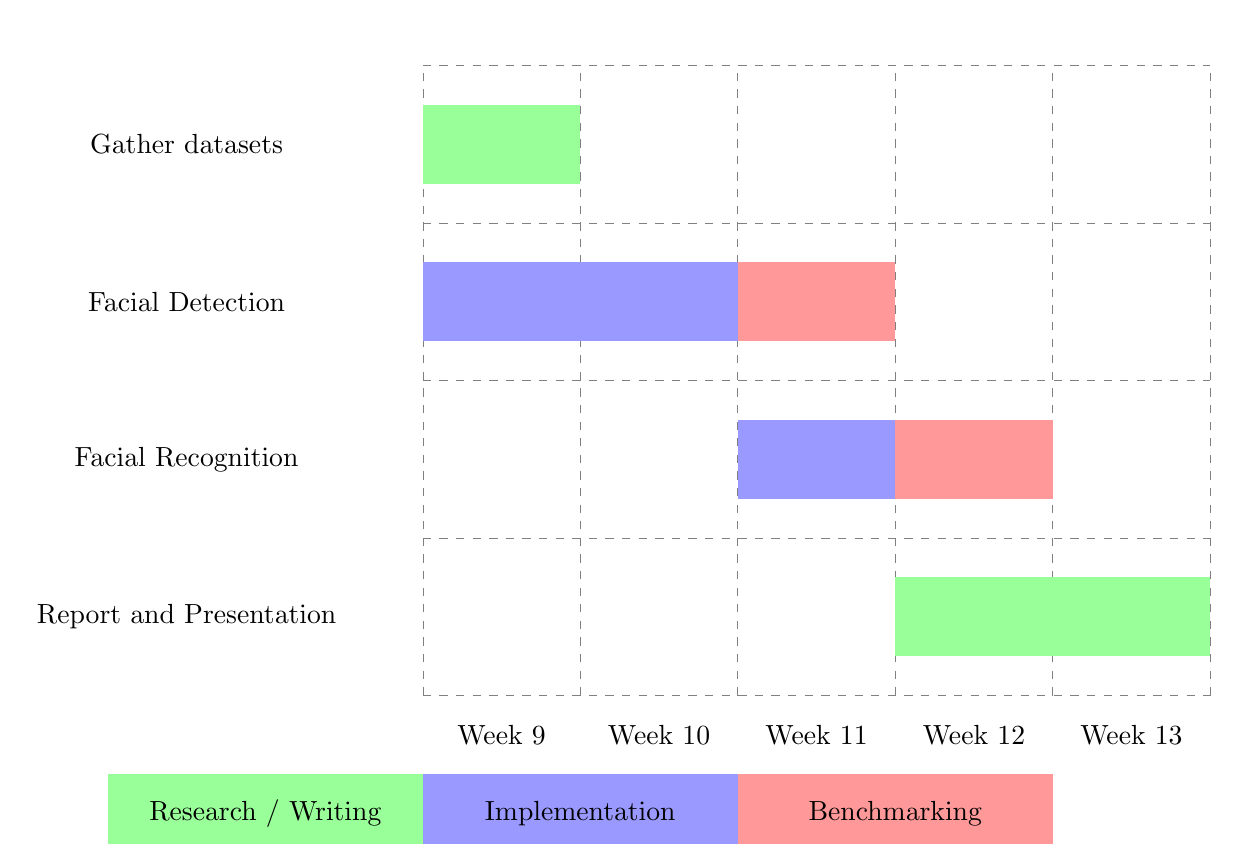
\begin{tikzpicture}[every node/.style={font=\normalsize,
  minimum height=0.5cm,minimum width=0.5cm},]

  \draw[step=2cm,gray,very thin,dashed] (0,0) grid (10,8);
  \node[] at (1,-0.5) {Week 9};
  \node[] at (3,-0.5) {Week 10};
  \node[] at (5,-0.5) {Week 11};
  \node[] at (7,-0.5) {Week 12};
  \node[] at (9,-0.5) {Week 13};

  % datasets
  \node[] at (-3, 7) {Gather datasets};
  \fill[green!40!white] (0,6.5) rectangle (2,7.5);

  % SIFT feature detection + Eigen faces  
  \node[] at (-3, 5) {Facial Detection};
  \fill[blue!40!white] (0,4.5) rectangle (4,5.5);
  \fill[red!40!white] (4,4.5) rectangle (6,5.5);

  % ranking
  \node[] at (-3, 3) {Facial Recognition};
  \fill[blue!40!white] (4,2.5) rectangle (6,3.5);
  \fill[red!40!white] (6,2.5) rectangle (8,3.5);

  % documentation
  \node[] at (-3, 1) {Report and Presentation};
  \fill[green!40!white] (6,0.5) rectangle (10,1.5);

  % legend
  \fill[green!40!white] (-4, -2) rectangle (0, -1);
  \node[] at (-2, -1.5) {Research / Writing};
  \fill[blue!40!white] (0, -2) rectangle (4, -1);
  \node[] at (2, -1.5) {Implementation};
  \fill[red!40!white] (4, -2) rectangle (8, -1);
  \node[] at (6, -1.5) {Benchmarking};

\end{tikzpicture}
\end{figure}
\bibliography{document}

%----------------------------------------------------------------------------------------

\end{document}